\documentclass[a4paper, 12pt, onecolumn, openright, oneside]{report}

\usepackage[utf8]{inputenc}
\usepackage[pdftex]{graphicx}
\usepackage{setspace}
\usepackage[T1]{fontenc}
\usepackage[francais]{babel}
\usepackage{color}
\usepackage{enumitem}
\usepackage{graphicx}
\usepackage{fancybox}
\usepackage{color}
\usepackage{geometry}
\usepackage{comment}
\usepackage{lipsum}
\usepackage[french]{minitoc}
\usepackage[nottoc]{tocbibind}
\usepackage[nottoc]{tocbibind}
\usepackage{fancyhdr} %pour definir les entêtes et pied de pages
\usepackage[Sonny]{fncychap} %style de chapitre
\usepackage{caption} %caption des images figure
\usepackage{epigraph} %citations%
\usepackage{lmodern}
\usepackage{tikz}
\usepackage{pict2e} %shéma%
\pagestyle{fancy}
\fancyhead[C]{}
\fancyhead[L]{\leftmark}
\fancyhead[R]{}
\definecolor{rouge}{RGB}{255,112,119}
\definecolor{rouge-clair}{RGB}{255,163,168}
\definecolor{rouge-tres-clair}{RGB}{255,217,219}
\newcommand{\hr}{\rule{\linewidth}{0.5mm}}
\newcommand{\br}{\\[0.5cm]}
\renewcommand*{\familydefault}{\sfdefault}
%Numéro de sections dans la marge
\makeatletter
\def\@seccntformat #1{ %
\protect\makebox[0pt][r]{\csname the#1\endcsname \quad }}
\makeatother
\captionsetup{
font=footnotesize,
justification=raggedright,
singlelinecheck=false
}
\usepackage{xcolor}
\usepackage{adjustbox}

\newenvironment{colbox}[2]{%
    \begin{adjustbox}{minipage=[b]{380px},margin=1ex,bgcolor=#1,env=center}% or use `bgcolor={HTML}{#1}` if you want to force HTML colors
        \textbf{#2}\\
}{%
    \end{adjustbox}%
}

\begin{document}
  \begin{titlepage}
  \begin{minipage}[t]{7cm} %t = top%
    \flushleft 
\includegraphics[width = 5cm]{images/logo_istic.png}
  \end{minipage}
  \hfill
  \begin{minipage}[t]{7cm}
    \flushright 
\includegraphics[width = 5cm]{images/logo_capgemini.png}
  \end{minipage}
  \\[2cm]
  \begin{center}
    \hr\\[0.5cm]
    {\huge\textbf{Rapport de stage }}\\[0.4cm]
    {\large\textbf{Développeur sur le projet Geofibre}}\\[0.4cm]
    \hr\\[0.5cm]
    \textsc{Thibault Gauthier\footnote{Mise à jour le \today}}\\[0.4cm]
    Du 9 Mars au 28 Août 2015\\[2.5cm]
  \end{center}
  \begin{minipage}[t]{8cm} %t = top%
    \textbf{Tuteur en entreprise}\\
    \textsc{Monsieur Patrick VEILLON}\\[0.5cm]
    \textbf{Tuteur académique}\\
    \textsc{Monsieur François POULET}
  \end{minipage}
  \hfill
  \begin{minipage}[t]{8cm}
    \textbf{Entreprise d'accueil} \\
    \textsc{Capgemini}\\
    \textit{7 Rue Claude Chappe\\
    35510 Cesson-Sévigné}\\[0.5cm]
    \textbf{\'Etablissement de formation}\\
    \textsc{ISTIC\footnotemark}\\
    \textit{263 avenue du Général Leclerc\\
    35042 Rennes}\\[0.5cm]
    \textbf{Intitulé de la formation}\\
    \textsc{Master MIAGE\footnotemark}

  \end{minipage}
  %en dehors de l'env minipage
  \addtocounter{footnote}{-2} %3=n
  \stepcounter{footnote}\footnotetext{Unité de formation en informatique et électronique à l'université de Rennes 1}
  \stepcounter{footnote}\footnotetext{Méthodes informatiques appliquées à la gestion des entreprises}

\end{titlepage}

  %-------------------------------------------------------%
  \chapter*{Remerciements}
\begin{flushright}
Je tiens à remercier toutes les personnes qui ont contribué au bon déroulement de mon stage.
\\En premier lieu Monsieur \textsc{Patrick Veillon}, Madame \textsc{Anne-Sophie Lescop} ainsi que l'entreprise Capgemini
qui m'ont donné l'opportunité et accordé leur confiance pour réaliser mon stage de fin d'études.
\\Je remercie également Monsieur \textsc{Jérome le Dorze}, Monsieur \textsc{Gaëtan Vieau} et toute l'équipe du projet Geofibre (\textsc{Omar, Olivier, Xavier, Jalal, Gaël, Sébastien, Damien, Taher}) pour leur aide et leurs conseils tout au long du stage.
\\Pour finir, je tiens à manifester ma gratitude à Messieurs \textsc{Mickaël Foursov, Charles Queguiner, François Poulet et Didier Certain} ainsi qu'à l'ensemble des enseignants pour le bon déroulement de ces trois années du cursus MIAGE.
\end{flushright}

  %-------------------------------------------------------%
  \setcounter{secnumdepth}{1} %pas de numérotation des subsections
  \setcounter{tocdepth}{1}  %pas de numérotation des subsections
  \tableofcontents
  %-------------------------------------------------------%
  \chapter*{Introduction}
\addstarredchapter{Introduction}
La fin du master \textit{MIAGE} se concrétise par la réalisation d’un stage en entreprise d’une durée de 6 mois.
\\J’ai choisi de réaliser ce stage au sein de l’entreprise \textsc{Capgemini} du 9 mars au 21 août 2015,
dans le centre de services \textit{TMA OSS}\footnote{Tierce Maintenant Applicative des applications orientés réseau d'Orange} à Rennes.
\\Mon choix s’est porté sur ce stage pour plusieurs raisons.
 Tout d’abord la présentation du sujet m'a séduit, le projet \textit{Geofibre} m'a beaucoup plu.
 Ensuite, mes différentes expériences de stage ayant jusqu’alors été réalisées en
autonomie ou en binôme, je souhaitais intégrer une équipe de travail déjà en place.
\\Pour finir, je n'ai encore jamais travaillé dans une \textit{ESN}\footnote{Entreprise de services du numérique}, c'était l'occasion de se
faire une opinion.
\\\\
Dans un premier temps je présenterai le contexte du stage, l'entreprise d'accueil et le projet sur lequel j'ai travaillé.
Puis, dans un second temps je présenterai le stage en lui-même.

  %-------------------------------------------------------%
  \part{Contexte du stage}
  \chapter{La société Capgemini}
\subsection*{Introduction}
Capgemini est une ESN\footnote{Entreprise de services du numérique} multinationale spécialisée dans le génie logiciel.
\\Elle a été créee le 1er Octobre 1967 à Grenoble par Monsieur \textsc{Serge Kampf} et elle est actuellement dirigée par  Monsieur \textsc{Paul Hermelin}.\\
En France, elle est la première dans son domaine en terme de chiffre d'affaire. \'A l'internationale, elle figure parmi les cinq premiers.
\\Capgemini est notamment côtée en bourse au CAC40.
\\\\
\begin{figure}[h]
  \captionbox{Monsieur Serge KAMPF\label{fig:dummy}}{
    
\includegraphics[width=4cm]{images/sergekampf.png}
  }
  \captionbox{Monsieur Paul HERMELIN\label{fig:dummy}}{
    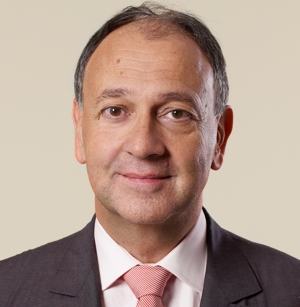
\includegraphics[width=4cm]{images/paulhermelin.png}
  }
  \captionbox{Logo de Capgemini\label{fig:dummy}}{
    
\includegraphics[width=5cm]{images/logo_capgemini.png}
  }
\end{figure}

\newpage
\section{Fiche d'identité}
\begin{description}
  \item[Raison sociale] : Capgemini
  \item[Année de création] : 1967
  \item[Fondateur] : Serge Kampf
  \item[Forme juridique] : Société anonyme à conseil d'administration
  \item[Siège social] : Paris
  \item[Directeur Général] : Paul Hermelin
  \item[Présence internationale] : 40 pays
  \item[Effectif en 2014] : 145 000
  \item[Chiffre d'affaire en 2014] : 10,6 milliards d'euros
\end{description}
\begin{figure}[h]
  \captionbox{Chiffre d'affaire par pays (2014)\label{fig:dummy}}{
    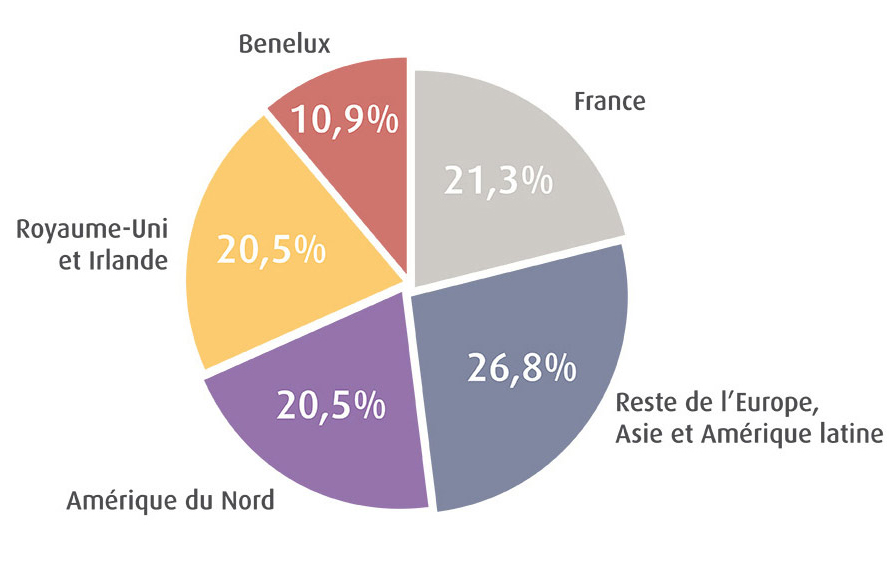
\includegraphics[width=15cm]{images/capays.png}
  }
\end{figure}
\newpage
\section{Métiers et activités}
\subsection{Secteurs d'activités}
Capgemini est spécialisé dans 6 secteurs d'activités :
\\
\begin{enumerate}
\item \textbf{Télécom, Média et \textit{Entertainment}}
\item \textbf{\'Energie, \textit{utilities} et chimie.}
\item \textbf{Industrie manufacturière et pharmaceutique}
\item \textbf{Services financiers}
\item \textbf{Grande consommation, distribution, transport et logistique}
\item \textbf{Services publics}\\
\end{enumerate}
\begin{figure}[h]
  \captionbox{Chiffre d'affaire par secteur (2014)\label{fig:dummy}}{
    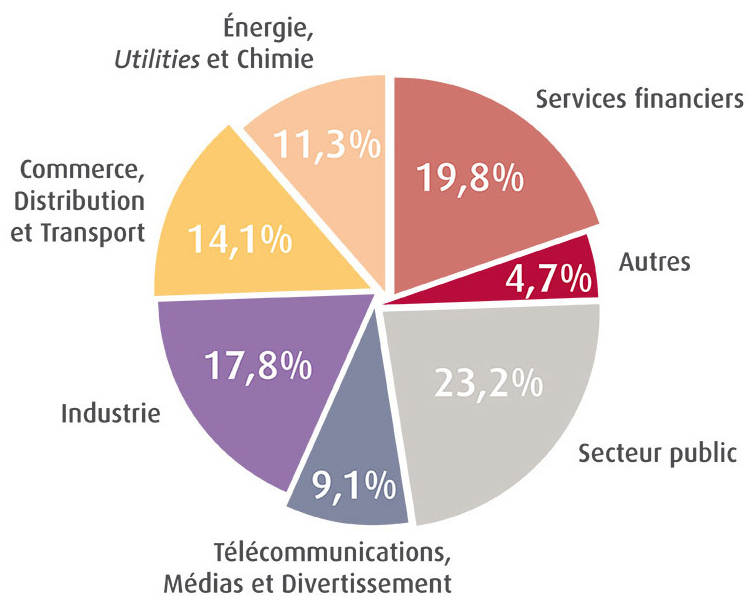
\includegraphics[width=12cm]{images/casecteur.png}
  }
\end{figure}
\newpage
\subsection{Métiers}
Capgemini travail dans 4 métiers principaux :
\\
\begin{enumerate}
\item \textbf{Le conseil en management (Capgemini Consulting)} a pour mission de contribuer, au travers d’actions telles que la transformation de l’activité ou la redéfinition de grandes fonctions, à l’amélioration des performances économiques des entreprises, grâce à une connaissance approfondie de leurs métiers et de leurs processus.
\item \textbf{L'intégration de systèmes et le développement d'applications} fait appel à la capacité de concevoir et d’intégrer des solutions, d’exploiter les innovations et de transformer l’environnement technologique.
\item \textbf{L’infogérance (Outsourcing Services - OS)} se concrétise par une prise en charge totale ou partielle de la gestion des ressources informatiques du client. Le Groupe a développé une gamme de services de gestion de systèmes informatiques, d’optimisation des processus métiers et de flexibilité des coûts de structures afin d’améliorer le rapport coût/performance.
\item \textbf{L'assistance technique et services de proximité (Sogeti)} ) sont implantés géographiquement au plus près des décideurs techniques locaux des grandes entreprises, visant à soutenir les capacités internes des directions informatiques en leur proposant dans des délais les plus brefs les meilleurs spécialistes.
\end{enumerate}
\begin{figure}[h]
  \captionbox{Chiffre d'affaire par metiers (2014)\label{fig:dummy}}{
    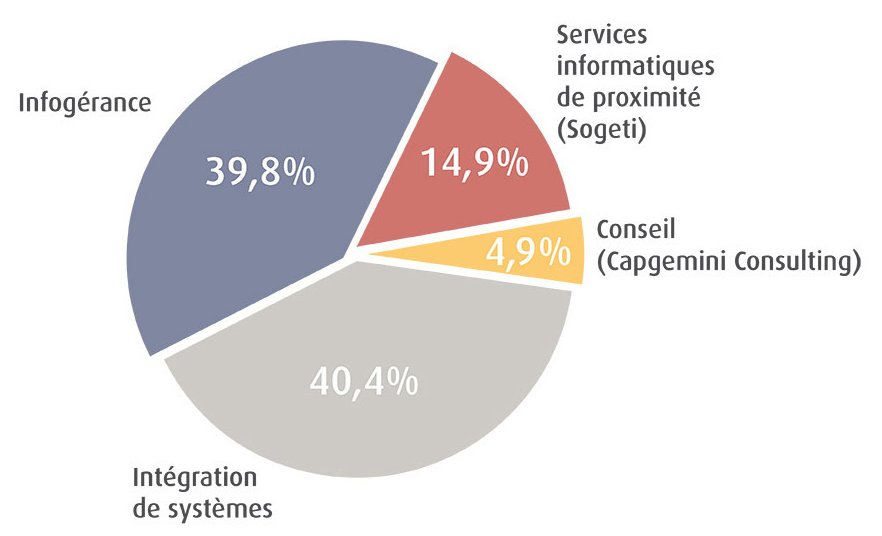
\includegraphics[width=13cm]{images/cametier.png}
  }
\end{figure}

  \chapter{Capgemini à Rennes}
\section{Fiche d'identité}
\begin{description}
  \item[Locaux] : Le Spiréa - Champs Blancs - Rennes
  \item[Année de construction] : 2012
  \item[Surface] : 9 850 m$^2$
  \item[Effectif en 2014] : 858
\end{description}
\begin{figure}[h]
  \captionbox{Le Spiréa à Rennes\label{fig:dummy}}{
    
\includegraphics[width=15cm]{images/spirea.jpg}
  }
\end{figure}
\newpage
\section{Secteurs d'activités}
Le site de Rennes est divisé en 4 secteurs :
\begin{enumerate}
\item Aérospatiale et Défense
\item \textbf{ADM\footnote{Application Development and Maintenance} Center}
\item Services
\item Télécom et Média\\
\end{enumerate}

\begin{colbox}{{HTML}{C7FF99}}{}
  Mon stage c'est déroulé dans la division \textsc{ADM Center}.\\
  Dirigé par Monsieur \textsc{Jean-Louis Hammon}
  cette division s'occupe de la maintenance et de l'évolution d'application logiciel.
\end{colbox}

\section{Le centre de service TMA OSS}

La division ADM Center est subdivisé en plusieurs centre de services dont le service TMA OSS\footnote{Tierce Maintenance des Applications OSS d’Orange}.
Dirigé par Monsieur \textsc{Arnaud Bellina} ce centre s'occupe de la maintenance des applications orientée réseau pour le client Orange.
Il répond à diverses missions :

\begin{enumerate}
\item Développement d'évolutions
\item Soutien et maintenance
\item Audit et architecture
\item Assistance\\
\end{enumerate}

TMA OSS a 60 applications en activités et il est réparti sur 5 domaines différents :

\begin{enumerate}
\item \textbf{SIG\footnote{Système d’information géographique }}
\item Déploiement et interventions
\item Supervision QoS\footnote{Quality of Service}
\item RTG+\footnote{Ready-To-Go+} Supervision\\
\end{enumerate}

\section{Le domaine de compétence SIG}
\textsc{
Un système d’Information Géographique est un outil informatique permettant de représenter et d’analyser toutes les choses qui existent sur terre ainsi que tous les événements qui s’y produisent.
}\\\\
Les SIG offrent toutes les possibilités des bases de données (telles que requêtes et analyses statistiques) et ce, au travers d’une visualisation unique et d’analyse géographique propres aux cartes.
\\Ces capacités spécifiques font du SIG un outil unique, accessible à un public très large et s’adressant à une très grande variété d’applications.
Les enjeux majeurs auxquels nous avons à faire face aujourd’hui (environnement, démographie, santé publique…) ont tous un lien étroit avec la géographie.
De nombreux autres domaines tels que la recherche et le développement de nouveaux marchés, l’étude d’impact d’une construction, l’organisation du territoire, la gestion de réseaux, le suivi en temps réel de véhicules, la protection civile… sont aussi directement concernés par la puissance des SIG pour créer des cartes, pour intégrer tout type d’information, pour mieux visualiser les différents scénarios, pour mieux présenter les idées et pour mieux appréhender l’étendue des solutions possibles.
\\Les SIG sont utilisés par tous ; collectivités territoriales, secteur public, entreprise, écoles, administrations, états utilisent les Systèmes d’Informations Géographique (SIG). La création de cartes et l’analyse géographique ne sont pas des procédés nouveaux, mais les SIG procurent une plus grande vitesse et proposent des outils sans cesse innovant dans l’analyse, la compréhension et la résolution des problèmes.
\\L’avènement des SIG a également permis un accès à l’information à un public beaucoup plus large.
\\\\
Aujourd’hui, les SIG représentent un marché de plusieurs milliards d'euros dans le monde et emploient plusieurs centaines de milliers de personnes.
\begin{flushright}
\textit{source : Esri France}
\end{flushright}

  \chapter{Le projet Géofibre}
\section{Objet}
Le projet \textit{Geofibre} a pour objet de fournir une application de \textit{SIG} pour \textsc{Orange} dans le domaine du \textit{FTTH}\footnote{Fiber To The Home : C'est le réseau trés haut débit de fibre optique pour les clients résidentiels.}.\\
L'application se présente sous la forme d'une page Web permettant de gérer et concevoir des données descriptives du réseau \textit{FTTH} en France Métropolitaine (\textit{et depuis peu dans les départements d'Outre-Mer}), en temps réel avec plusieurs utilisateurs connectés simultanément.\\
Cette application est principalement destinée aux chargés d'affaire et sous-traitant \textit{FTTH}.\\
Elle a pour mission, par exemple, de faire évoluer le réseau en permettant la conception sur l'application pour ensuite l'imprimer et l'installer sur le terrain ou par exemple avoir une vision globale des installations sur une commune.\\
En matière de charge, elle comptabilise en 2015 jusqu'à \textbf{1150 utilisateurs simultanés}.\\
Techniquement \textit{Geofibre} est basé sur le progiciel \textit{ArcGIS} de l'éditeur \textsc{ESRI}.

\newpage
\section{Historique}
Le lancement du projet a eu lieu en 2010. Jusqu'en 2012 le projet s'est développé dans les locaux du client dans la ville de Lannion suivant la méthode de gestion de projets \textit{AGILE}.\\
Les employés de la société \textsc{Capgemini} étaient à cette époque présents dans les locaux du client pour travailler en tant qu'assistants techniques.
Par la suite le développement du projet s'est réalisé dans les locaux de \textsc{Capgemini}, au \textit{Spirea} à Rennes.\\\\
Depuis ses débuts \textit{Geofibre} a évolué de manière significative. \'A l'heure actuelle le projet est à sa 7ème version mineure(cf.\ref{versionning}) et des évolutions sont prévues, d'autant que le gouvernement Français souhaite développer la fibre optique sur l'ensemble du territoire Français.

\section{Illustration}
\begin{figure}[h]
	\captionbox{Capture d'écran du projet Geofibre\label{fig:dummy}}{
		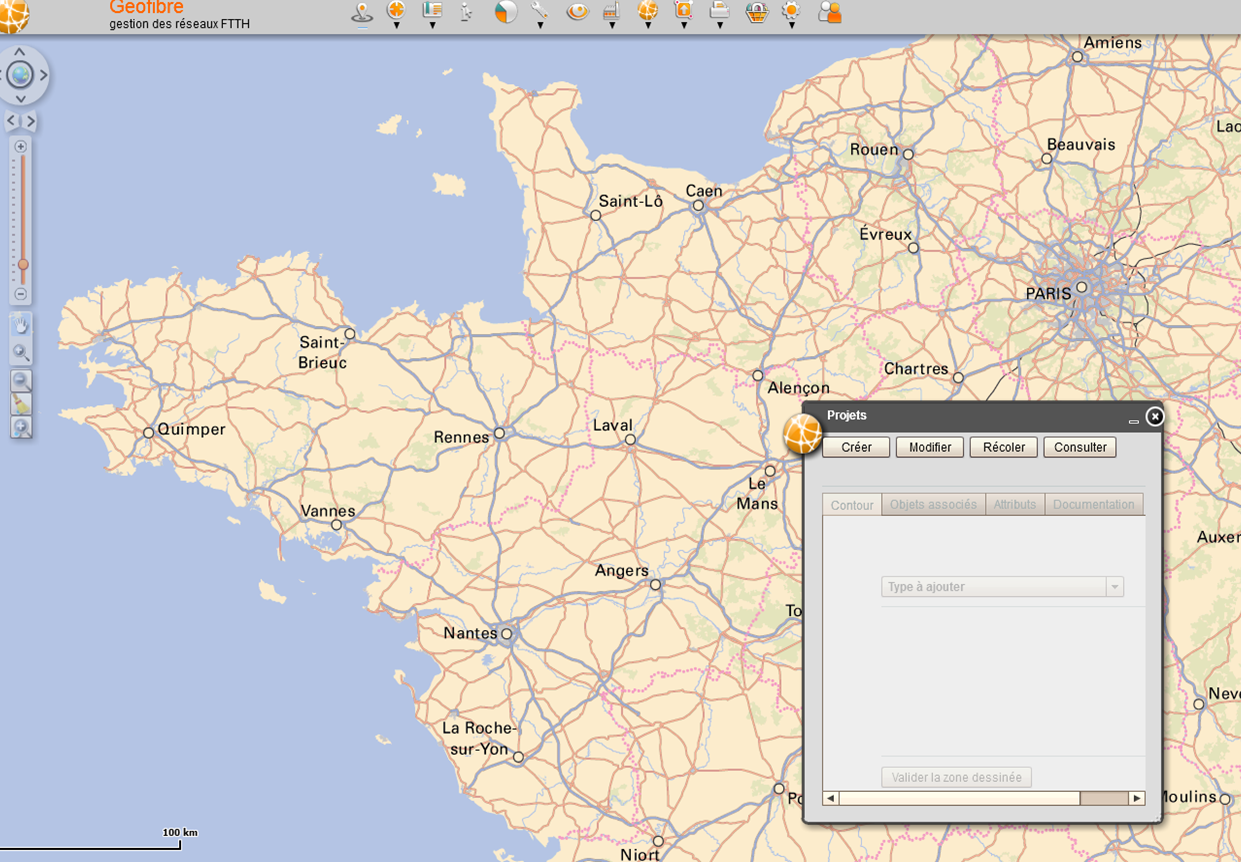
\includegraphics[width=16cm]{images/shotgeofibre.png}
	}
\end{figure}

  %-------------------------------------------------------%
  \part{Réalisation du stage}
  \chapter{Intégration dans l'équipe de projet}

\chapter{Montée en compétence}
Lorsque j'ai débuté mon stage je n'avais aucune visibilité sur le projet.
J'ai du me documenter et poser un tas de questions pour comprendre comment été structuré le projet d'une part et comment il fonctionné d'autre part. Ensuite il m'a fallu comprendre comment se déroulé le processus de développement dans Capgemini.
Cette phase de montée en compétence s'est déroulé tout au long du stage.

\section{Configuration du projet}
\subsection{Identification des versions}
\label{versionning}
Les versions sont marquées par des labels qui doivent permettre d'identifier de façon non équivoque toutes les évolutions successives des composants pour pouvoir retrouver et extraire de la base d'archives toute version livrée au client ou livrée pendant les phases d'intégration ou de la validation interne.
\\\\
On distingue deux types de versions :
\begin{description}
	\item[Version majeure] : c'est une version complète du logiciel, c'est à dire qu'elle contient l'ensemble des composants du système
	\item[Version mineure] : c'est une version paertielle du logiciel, c'est à dire qu'elle ne contient qu'un sous-ensebmel des composants du système, qui constitue un delta par rapport à la version précédente
	(qui peut être une version majeure ou mineure) ; c'est en général le résultat d'une correction ou d'une évolution mineure.
\end{description}
Les labels de version sont structurés de telle sorte que cette dépendance entre versions soit mise en évidence.
\\La composition d'un label de version est de la forme \textsc{GxxRyyCzz}.
\\Dans ce sigle on retrouve :
\begin{description}
	\item[Révision] : Une révision est attachée à un composant. \'A chaque fois qu'un utilisateur archive une nouvelle version d'un composant, l'outil de gestion de configuration crée une nouvelle révision de ce composant.
	\item[Version et labels] : Une version permet d'identifier un ensemble cohérent de composants d'une application. L'identifiant de version est sous contrôle complet de l'équipe de projet. Par exemple la première version est la G1R0C0, puis les suivantes seront les
	G1R1C0 puis la G2R0C0.
	\item[Tronc et branches] : Le \textit{tronc} supporte les versions principales. En cas de travaux parallèles sur plusieurs versions (par exemple la correction d'une anomalie sur une version n-1 et développement de la version n), on crée une branche qui va permettre de modifier une version déjà livrée.
	\\
\end{description}
\textbf{Exemple} : La branche G1R0 contient les versions correctives G1R0C1 et G1R0C2 qui intégrent des correctifs d'anomalies idnetifiées sur la version G1R0C0 préalablement livrée.
\setlength{\unitlength}{1.3cm}

\begin{picture}(5,5)
	%texte
	\put(-2,4.4){Tronc}
	\put(-2,2.4){Branche G1R0}
	%traits haut
	\put(2.5,4.4){\vector(1,0){1.5}}
	\put(6.5,4.4){\vector(1,0){1.5}}
	\put(10.5,4.4){\vector(1,0){1.5}}
	%oblique
	\put(1.5,4){\vector(0.3,-1){0.5}}
	%traits bas
	\put(4.5,2.4){\vector(1,0){1.5}}


	\put(0,4){\framebox(2.5,0.8)[c]{G1R0C0}}
	\put(4,4){\framebox(2.5,0.8)[c]{G1R1C0}}
	\put(8,4){\framebox(2.5,0.8)[c]{G2R0C0}}

	\put(2,2){\framebox(2.5,0.8)[c]{G1R0C1}}
	\put(6,2){\framebox(2.5,0.8)[c]{G1R0C2}}
\end{picture}
\begin{colbox}{{HTML}{C7FF99}}{}
Durant mon stage j'ai participé à l'intégration de la 6ème version (G1R6C0) et au développement et à l'intégration de la 7ème version (G1R7C0).
\end{colbox}

\newpage

\subsection{Organisation des environnements de travail}

Le \textbf{référenciel} (\textit{Repository}) contient l'ensemble des révisions de chaque composant ainsi que les liens entre composants permettant d'identifier les versions successives de chaque application.
\\\\
Les \textbf{espaces de travail} (\textit{Workspaces}) sont les espaces utilisés pour développer, intégrer, valider et livrer chaque application.
\\
\begin{picture}(0,1)
	%Referenciel
	\put(0,-2){Référenciel}
	\put(0.7,-1.5){\oval(2,2)[t]}
	\put(-0.3,-2.5){\line(0,1){1}}
	\put(1.7,-2.5){\line(0,1){1}}
	\put(0.7,-2.5){\oval(2,2)[b]}
	%fleches
	\put(1.7,-1.5){\vector(1,0){6}}
	\put(2.6,-1.4){Extraction des composants}

	\put(7.7,-2.5){\vector(-1,0){6}}
	\put(2.6,-2.4){Archivage des composants}
	%espaces de travail x+8
	\put(7.8,-2){Espaces de travail}
	\put(8.2,-2.6){Composants}
	\put(8.7,-1.5){\oval(2,2)[t]}
	\put(7.7,-2.5){\line(0,1){1}}
	\put(9.7,-2.5){\line(0,1){1}}
	\put(8.7,-2.5){\oval(2,2)[b]}
	%+0.3
	\put(9,-1.5){\oval(2,2)[t]}
	\put(8,-2.5){\line(0,1){1}}
	\put(10,-2.5){\line(0,1){1}}
	\put(9,-2.5){\oval(2,2)[b]}

	\put(9.3,-1.5){\oval(2,2)[t]}
	\put(8.3,-2.5){\line(0,1){1}}
	\put(10.3,-2.5){\line(0,1){1}}
	\put(9.3,-2.5){\oval(2,2)[b]}

\end{picture}
\\[6cm]
Quand l'activité le justifie, il est possible de devoir travailler simultanément sur plusieurs versions, en général :
\begin{itemize}
	\item Une version en \textbf{développement}
	\item Une version en \textbf{maintenance}\\
\end{itemize}
Il faut donc prévoir autant d'espaces de travail disponibles et ceci pour les différentes phases du cycle de développement :
\begin{itemize}
	\item Développement et tests unitaires
	\item Intégration et validation
	\item Livraison (effectuée sur la palte-forme de qualification)
\end{itemize}

\section{Cycle de développement}

Le développement se déroule en cycle en V :
%\begin{description}
  %\item[Spécifications] Le prestataire et le client communique pour valider les spécifications de la version.
  %\item[Chiffrage] Le prestataire fait un chiffrage et convient notamment des délais de livraison.
  %\item[Répartition des tâches] Le chef de projet répartie les tâches en fonction des domaines de compétence et de manière équilibré entre les développeurs.
  %\item[Développement] Les développeurs réalise les tâche demandées en suivant les spécifications.
  %\item[]



\section{Architecture du projet}
\subsection{Architecture technique}
L'architecture technique repose sur des machines virtuelles (excepté la BDD).
Voici une liste des infreastructures présentes :
\begin{description}
	\item[Serveur WAS] C'est le serveur qui délivre l'application à l'utilisateur. En effet, il s'y connecte via le GASSI du client avec le protocole HTTP ou via un VPN avec le protocole SSL. Il fonctionne sur une machine Linux avec le serveur d'application JOnAS\footnote{Java Open Application Server}.
\item[Serveur ArcGIS] Il traite les données SIG via le serveur ArcGIS délivré par l'éditeur Esri. Il fait le pont entre le serveur de base de données et le serveur WAS et accède aussi, via une architecture REST et SOAP à des interfaces Externes pour diverses missions. Par exemple avec l'application \textit{SIGEO}, développé par Capgemini pour récupérer les \textit{tuiles} de fond de plan.
\item[Serveur d'impression] En raison de la charge induite par la génération des PDF destiné à l'impression de fond de plan (certains au format A0), des serveurs sont dédiés à cette tâche. Il fonctionne avec le serveur ArcGIS.
\item[Serveur de base de données] Le serveur de base de données est PostGreSQL et permet de gérer l'accès et le stockage des données.\\
\end{description}

\'Etant donné la charge sur l'application (rappel : 1150 utilisateur simultanés par jour) il existe plusieurs instances de serveurs et la communication d'un serveur à un autre se fait via des répartiteurs de charges qui vont requêter le bon serveur au bon moment afin d'équilibrer la charge de travail entre les différents serveurs. De ce fait il y a, en plateforme de production :

\begin{itemize}
	\item 3 Serveurs WAS
	\item 8 Serveurs ArcGIS pour la France Métropolitaine et 2 pour les DOM
	\item 1 Serveur de base de données
	\item 4 Serveurs d'impressions\\
\end{itemize}
Pour une meilleure visibilité, vous pourrez trouvez le shéma d'achitecture technique en annexe \ref{archtech}.

\subsection{Architecture logicielle}

Geofibre est composé de 4 briques logiciel :
\begin{description}
	\item[gfi-bdd] Ce projet est lié à la structure des données du projet et contient les différents scripts PostgreSQL, fonctions et vues du projet. Ainsi que les différentes données liées à la configuration.
	\item[gfi-expl] Ce projet est liés à l'exploitation des serveurs faisant tourner le projet. Il contient majoritairement des scripts liés à la configuration des serveurs, des droits d'utilisation.
	\item[gfi-front] Ce projet est lié à l'IHM de l'application. Il contient du code en langage ActionScript 3 compilé par Adobe Flex.
	\item[gfi-back] Ce projet est lié au backoffice de l'application. Il contient du code Java tournant sur un serveur afin de requêter en REST et SOAP le serveur ArcGIS.
\end{description}
\begin{figure}[h]
	\captionbox{Arborescence du projet Geofibre\label{fig:dummy}}{
	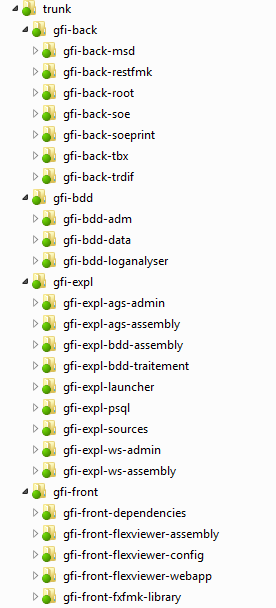
\includegraphics[width=7cm]{images/arborescence.png}
	}
\end{figure}
\chapter{Version G1R6C0}
Je suis arrivbé en cours de dev
\section{Spécifications}
\section{Développement}
\section{Rédaction des tests unitaires}
\section{Qualité de code}
\section{Intégration}
vague d'intégrationjusqu'il n'y a plus d'ano critiques
\subsection{Tests d'intégration des DOM}
\subsection{Tests de non-régression de la France Métropolitaine}
\subsection{Correction d'anomalies}

\chapter{Maintenance}
Pendant la phase de spécifications de la G1R7
\section{Correction d'anomalies éligibles à la G1R7}


\chapter{Version G1R7C0}
Cette version est essentiellement  fonctionnelle et dédiée à la prise en compte des paliers RIP et DSP.
Détail des items embarqués :
\begin{itemize}
\item Migration des RIP LTHD et CAPS de TIGRE
\item Configuration d’un ensemble de RIP
\item Gestion de valeurs par défaut sur l’IHM pour faciliter les actions de création/modification
\item Prise en compte des impacts sur les interfaces avec IPON (dont flux supplémentaires)
\item Prise en compte des impacts sur la Publication du SD.
\item Prise en compte des impacts sur la symbologie des immeubles
\item Ajout de filtrages RIP/Orange
\item Mise en conformité des études RIP existantes dans Geofibre
\item	Enveloppe MCO de la DS PIAR
\item Modification de la définition des diamètres des câbles pour l'extraction de l'annexe C3a (avec table de correspondance).
\item Evolution réglementaire de l’Annexe D8 (exports OPGC afin de différencier le mode de pose (Aérien ou Souterrain) et de visualiser le nombre de câbles sur les parcours (dont information de mode de pose liée au parcours).
\item Changement d’identification sur les nouveaux appuis ERDF (Exxxxxx au lieu de ERDFxxx), sans rattrapage de l’existant.
\item Des utilisateurs spécialisés sur l’activité RIP vont être ajoutés sur l’IHM GeoFibre.
\end{itemize}
D’un point de vue technique, la seule évolution concerne les flux IPON->GFI : IPON enverra un fichier Orange et un fichier RIP pour les câbles et les points techniques.
Aucune autre incidence sur l’architecture : le nombre des  nouveaux utilisateurs n’est pas de nature à saturer les ressources serveurs.

\section{Spécifications}
\section{Développement}
\subsection{Exemple}
\section{Rework}
\subsection{Exemple}
\section{Intégration}

  %-------------------------------------------------------%
  \chapter*{Résumé}
\addstarredchapter{Résumé} 

  \chapter*{Abstract}
\addstarredchapter{Abstract}

My \textit{Master 2 MIAGE} internship was carried out within the company \textsc{Capgemini} at Rennes during six month.
\\\\
Within the service \textit{TMA OSS} I participated in the development and maintenance on \textit{Geofibre} application.
This application of \textit{GIS} enables business managers, via a \textit{web GUI}, to manage and develop the domestic \textit{FTTH} network in metropolitan France.
\\\\
My role was to provide the support to the development team for the integration of a new version of the application
to manage the \textit{FTTH} network of Overseas Departments ( French Guyana, Guadeloupe , Martinique and Réunion) .
Then, during the specification phase of the next release I spent to correct severals defects noted by the client.
Finally I participated in the development and integration of the latest version of the application that makes the management of new operators data.

  %-------------------------------------------------------%
  \chapter*{Conclusion}
\addstarredchapter{Conclusion}

Pour commencer le projet Geofibre est très intéressant de bout en bout et pour commencer m'a permis de découvrir le monde du SIG et du FTTH.
\\Techniquement j'ai pu découvrir le langage ActionScript et le framework Flex avec la programmation évenementiel même si c'est une technologie de moins en moins utilisée.
 \\ J'ai aussi pu découvrir le fonctionnement et l'utilité du progiciel ArcGIS.
 \\Aussi j'ai appris beaucoup de petites techniques de développement et de débuguage, notamment sur l'IDE Eclipse/FlashBuilder et en PostgreSQL.
\\\\Professionnellement cela m'a permis d'enrichir mon expérience et de mieux comprendre les différentes phases de déroulement d'un projet, ainsi que le développement et la méthodologie de travail dans un contexte industriel.
\\\\En ce qui concerne mon apport pour l'entreprise \textsc{Capgemini}, les évolutions développés et testés pour la version G1R6 ont été livrées à Orange et vont être utilisé en production.
\\\\Le stage m'a beaucoup apporté. J'ai travaillé avec une jeune équipe, qualifiée et compétente qui m'ont énormément aidé. J'ai pu apprendre, observer et acquérir de nouvelles compétences mais aussi apporter le fruit de mes années d'études au projet.

  %-------------------------------------------------------%
  \appendix
  \listoffigures
  \chapter{Bibliographie / Webographie}
\begin{description}
\item{[1]} [..]
\item{[2]} [..]
\item{[3]} [..]
\end{description} 
  \chapter{Carnet de bord des travaux r�alis�s par semaine}
\begin{enumerate}[label= Semaine \no\textbf{\arabic*.},itemsep=20pt]
\setcounter{enumi}{10}

\item \textbf{Visite, pr�sentation et rencontre} avec les �quipes de la ferme d'applications \textsc{TMA OSS\footnote{Tierce Maintenant Applicative des applications orient�s r�seau d'Orange}}. Explication de l'activit� par le chef de service \textsc{Arnaud Bellina}.
\newline Visite, pr�sentation et rencontre avec les diff�rents services du b�timent de Capgemini (Infirmerie, CE, Caf�taria, RH, Assistante) .
\newline \textbf{Installation de mon poste de travail} au sein de l'openspace de l'�quipe G�ofibre et int�gration supervis�e par le chef de groupe \textsc{Patrick Veillon} et la chef de projet \textsc{Anne-Sophie Lescop}.
\newline \textbf{Installation des logiciels} et \textbf{lecture} de la documentation ainsi que du code qui compose le projet G�ofibre �paul� par l'�quipe.

\item \textbf{Mont�e en comp�tence} g�n�rale sur l'application G�ofibre.
\item \textbf{D�veloppement de la version G1R6 Front (IHM Flex)} Externalisation des syst�mes de projection, emprise, �chelles, minimap

\item \textbf{D�veloppement de la version G1R6 Back (Serveur, Toolbox)} V�rification de la gestion de la projection

\item \textbf{D�veloppement de la version G1R6 Back (Serveur, Toolbox)} Aiguillage servlet
\newline \textbf{D�veloppement de la version G1R6 Back (Serveur, Toolbox)} Impact code appelant

\item \textbf{Tests d'int�gration de la version G1R6 sur la R�union}
\begin{enumerate}[label = Tests \no\arabic*.,align=left]
\item \emph{\colorbox{rouge}{P1}} - Gestion infrastructure - Recalage GC
\item \emph{\colorbox{rouge}{P1}} - Gestion infrastructure - Zone de recalage
\item \emph{\colorbox{rouge-clair}{P2}} - Exploitation - Import RCV (R�f�renciel Commune Voies)
\item \emph{\colorbox{rouge-clair}{P2}} - Localisation adresse
\item \emph{\colorbox{rouge-tres-clair}{P3}} - Purge des fichiers (multi instance)
\end{enumerate}

\item \textbf{Tests d'int�gration de la version G1R6 sur la Guyane}
\begin{enumerate}[label = Tests \no\arabic*.,align=left]
\item  \emph{\colorbox{rouge}{P1}} - Gestion FTTH - C�bles
\item \emph{\colorbox{rouge}{P1}} - Gestion FTTH - Parcours
\item\emph{\colorbox{rouge}{P1}} -  Gestion FTTH - Zone de travail
\item \emph{\colorbox{rouge}{P1}} - Gestion infrastructure - Itin�raires GC
\item \emph{\colorbox{rouge}{P1}} - Gestion infrastructure - Site supports
\item \emph{\colorbox{rouge-tres-clair}{P3}} - Filtrage
\item \emph{\colorbox{rouge-tres-clair}{P3}} - Gestion des droits
\item \emph{\colorbox{rouge-tres-clair}{P3}} - G�osignets
\item \emph{\colorbox{rouge-tres-clair}{P3}} - Outil de mesure
\item \emph{\colorbox{rouge-tres-clair}{P3}} - Sauvegarde du contexte
\item \emph{\colorbox{rouge-tres-clair}{P3}} - Table des mati�res
\end{enumerate}

\item \textbf{Tests d'int�gration de la version G1R6 sur la Guadeloupe}
\begin{enumerate}[label = Tests \no\arabic*.,align=left]
\item \emph{\colorbox{rouge}{P1}} - Gestion infrastructure - Site supports
\item \emph{\colorbox{rouge}{P1}} - Exports - Dossier OPGC - Base arri�re de PM
\item \emph{\colorbox{rouge-clair}{P2}} - M�j adresse des immeubles depuis optimum
\item \emph{\colorbox{rouge-clair}{P2}} - Exploitation - majBatchData
\item \emph{\colorbox{rouge-clair}{P2}} - Statistiques
\item \emph{\colorbox{rouge-tres-clair}{P3}} - Filtrage
\item \emph{\colorbox{rouge-tres-clair}{P3}} - Gestion des droits
\item \emph{\colorbox{rouge-tres-clair}{P3}} - G�osignets
\item \emph{\colorbox{rouge-tres-clair}{P3}} - Localisation objet m�tier
\end{enumerate}

\item \textbf{Tests d'int�gration de la version G1R6 sur la Martinique}
\begin{enumerate}[label = Tests \no\arabic*.,align=left]
\item  \emph{\colorbox{rouge}{P1}} - Gestion FTTH - C�bles
\item \emph{\colorbox{rouge}{P1}} - Gestion FTTH - Parcours
\item \emph{\colorbox{rouge}{P1}} - Gestion infrastructure - Itin�raires GC
\item \emph{\colorbox{rouge}{P1}} - Gestion FTTH - Projets
\item \emph{\colorbox{rouge}{P1}} - Gestion FTTH - Sch�ma directeur
\item \emph{\colorbox{rouge}{P1}} - Gestion FTTH - R�gles d'ingienerie
\item \emph{\colorbox{rouge}{P1}} - D�calages horaires
\item \emph{\colorbox{rouge-clair}{P2}} - Statistiques
\item \emph{\colorbox{rouge-tres-clair}{P3}} - Filtrage
\item \emph{\colorbox{rouge-tres-clair}{P3}} - Gestion des droits
\item \emph{\colorbox{rouge-tres-clair}{P3}} - Outil de mesure
\item \emph{\colorbox{rouge-tres-clair}{P3}} - Sauvegarde du contexte
\end{enumerate}
\textbf{Prise en main du logiciel ArcMap de la suite ArcGis.}
\item \textbf{Tests de non-regression de la version G1R6 sur la France m�tropolitaine}
\begin{enumerate}[label = Tests \no\arabic*.,align=left]
\item  \emph{\colorbox{rouge}{P1}} - Impression
\end{enumerate}
\textbf{Anomalie relev� sur les zones d'�gilibilit�s}
\newline
\textbf{Formation E-Learning}
\begin{enumerate}[label = Formation \no\arabic*.,align=left]
	\item \textit{Utiliser efficacement l'email et la messagerie isntantanee}
	\item \textit{Utiliser le Brown Paper}
	\item \textit{Utiliser du Portail MyLearning}
\end{enumerate}
\item \textbf{Tests de non-regression de la version G1R6 sur la France m�tropolitaine}
\begin{enumerate}[start = 2,label = Tests \no\arabic*.,align=left]
\item  \emph{\colorbox{rouge}{P1}} - Gestion FTTH - C�bles
\item  \emph{\colorbox{rouge}{P1}} - Gestion FTTH - R�gles d'ingienerie
\end{enumerate}
\textbf{Formation E-Learning}
\begin{enumerate}[label = Formation \no\arabic*.,align=left]
	\item \textit{Les fondamentaux du test logiciel}
\end{enumerate}

\newpage
\item \textbf{Pr�sentation du d�roulement de mon stage} Collecte d'informations sur le centre de service  \textsc{TMA OSS\footnote{Tierce Maintenant Applicative des applications orient�s r�seau d'Orange}} et le domaine de comp�tence \textsc{SIG\footnote{Syst�me d'Information G�ographique}} auquel se rattache le projet G�ofibre sur lequel j'effectue mon stage. Cr�ation d'un diaporama pour cette pr�sentation. R�alisation de la pr�sentation avec une dizaine de stagiaires, la responsable DRH et les diff�rents chefs de projets.
\newline
\textbf{Formation E-Learning}
\begin{enumerate}[label = Formation \no\arabic*.,align=left]
	\item \textit{La politique anti-corruption du groupe}
	\item \textit{Les lois de la concurrence}
	\item \textit{Les normes �cologique du groupe}
	\item \textit{Le code �thique dans la relation client}
\end{enumerate}
\item
\textbf{Correction d'anomalies hors-garantie �ligibles pour la version G1R7}
\textbf{Redaction et passage des \textsc{TU\footnote{Tests Unitaires}} relatifs aux corrections}
\begin{enumerate}[label = Correction \no\arabic*.,align=left]
	\item \textit{Repositionnement d'immeubles en masse} - Perte de la s�lection d'immeubles apr�s avoir annul� une fen�tre de choix d'immeuble.
	\item \textit{Repositionnement d'immeubles s�quentiel} - Perte de la s�lection d'immeubles apr�s avoir annul� une fen�tre de choix d'immeuble.
	\item \textit{Visu Shape} - Message d'erreur a tord "Le nombre maximum de fichiers visualis�s simultan�ment est de 5".
\end{enumerate}
\textbf{Formation E-Learning}
\begin{enumerate}[label = Formation \no\arabic*.,align=left]
	\item \textit{Communiquer avec assurance}
	\item \textit{Entretenir de bons rapports avec le client}
\end{enumerate}

\item
\textbf{Correction d'anomalies hors-garantie �ligibles pour la version G1R7}
\textbf{Redaction et passage des \textsc{TU\footnote{Tests Unitaires}} relatifs aux corrections}
\begin{enumerate}[label = Correction \no\arabic*.,align=left]
	\item \textit{Sites supports} - Perte d'information du champs gestionnaire lors de la duplication si celui-ci a la valeur "39" en production. (en attente d'informations d'Orange)
	\item \textit{C�bles, alv�oles} -  Suppression des donn�es d'alv�oles non homog�ne (en attente d'informations d'Orange)
\end{enumerate}
\textbf{Formation E-Learning}
\begin{enumerate}[label = Formation \no\arabic*.,align=left]
	\item \textit{El�ments d�une �quipe soud�e}
	\item \textit{Etablir des relations de confiance}
	\item \textit{Etre un membre efficace au sein d�une �quipe}
\end{enumerate}
\textbf{Breizhcamp}
\item
\textbf{Correction d'anomalies hors-garantie �ligibles pour la version G1R7}
\textbf{Redaction et passage des \textsc{TU\footnote{Tests Unitaires}} relatifs aux corrections}
\begin{enumerate}[label = Correction \no\arabic*.,align=left]
	\item \textit{Connexion} -  Geofibre ne g�re pas la casse du cu\_id d'un utilisateur.
	\item \textit{Impression Libre et Casage} - Perte de la valeur par d�faut du champ R�solution
\end{enumerate}
\textbf{Formation E-Learning}
\begin{enumerate}[label = Formation \no\arabic*.,align=left]
	\item \textit{Limitation des voleurs de temps}
	\item \textit{Contr�ler son stress}
	\item \textit{Planifier et hierarchiser son temps}
\end{enumerate}
\item
\textbf{Support � Taher qui viens d'arriver sur le projet}\\
\textbf{Correction d'anomalies hors-garantie �ligibles pour la version G1R7}\\
\textbf{Redaction et passage des \textsc{TU\footnote{Tests Unitaires}} relatifs aux corrections}\\
\begin{enumerate}[label = Correction \no\arabic*.,align=left]
	\item \emph{\colorbox{rouge}{majeure}} \textit{Flux cables} -  Echec de l'import sur pr�sence de point virgule , simple guillement ou double guillemet
\end{enumerate}
\textbf{D�tection de la version d'anomalie}\\
Certaines anomalies sont en garantie (versions G1R4, G1R5, G1R6) dans quel cas si le client les trouve il faudra les corriger.
D'autres sont hors-garantie (< G1R4) Dans ce cas il faut les annoncer aux clients et ils d�cident si ils veulent les corriger ou non.
\\
Pour cela il faut d�tecter ou est-ce que l'anomalie est situ�e dans le code et voir � quel moment les changements ont �t� commit� sur le gestionnaire de version SVN. En fonction de la date du commit ou du TAG
ont peut remonter au num�ro de version.
\begin{enumerate}[label = D�tection de la version d'anomalie \no\arabic*.,align=left]
	\item \textit{Points techniques} - Il est possible cr�er un PT avec une r�f�rence de plus de 25 caract�res
	\item \textit{Points techniques} - Import - Probl�me d'encodage dans les comptes rendus
\end{enumerate}
\textbf{Correction d'anomalies hors-garantie �ligibles pour la version G1R7}\\
\textbf{Redaction et passage des \textsc{TU\footnote{Tests Unitaires}} relatifs aux corrections}
\begin{enumerate}[label = Correction \no\arabic*.,align=left]
	\item \textit{Recalcul nombre d'EL} -majBatchData.ksh,KO si  la zone est � cheval sur deux communes [ksh, SQL, PostGIS]
\end{enumerate}
\textbf{Les sp�cifications de la version G1R7 ont �t� livr� et valid�. Les d�veloppements peuvent commencer !}
\item
\textbf{G1R7} Lecture assidu des sp�cifications\\
\textbf{G1R7} D�veloppement - [Site support] Ajout du champs d�ployeur en BDD\\
\textbf{Correction d'anomalies hors-garantie �ligibles pour la version G1R7}\\
\textbf{Redaction et passage des \textsc{TU\footnote{Tests Unitaires}} relatifs aux corrections}
\begin{enumerate}[label = Correction \no\arabic*.,align=left]
	\item \textit{Visu Shape} -sauvegarde dans le contexte utilisateur d'un shape non valide [IHM]
\end{enumerate}
\textbf{G1R7} D�veloppement - [Site support] Ajout du champs d�ployeur dans l'IHM\\
\item
\textbf{G1R7} D�veloppement - [Annexe C3A] Nouvelle gestion du diam�tre des parcours
\item
\item
\item
\item
\item
\item
\item
\item
\end{enumerate}

  \chapter{Shéma d'architecture technique}
\label{archtech}

\begin{figure}[h]
  \captionbox{Shéma d'architecture technique\label{fig:dummy}}{
    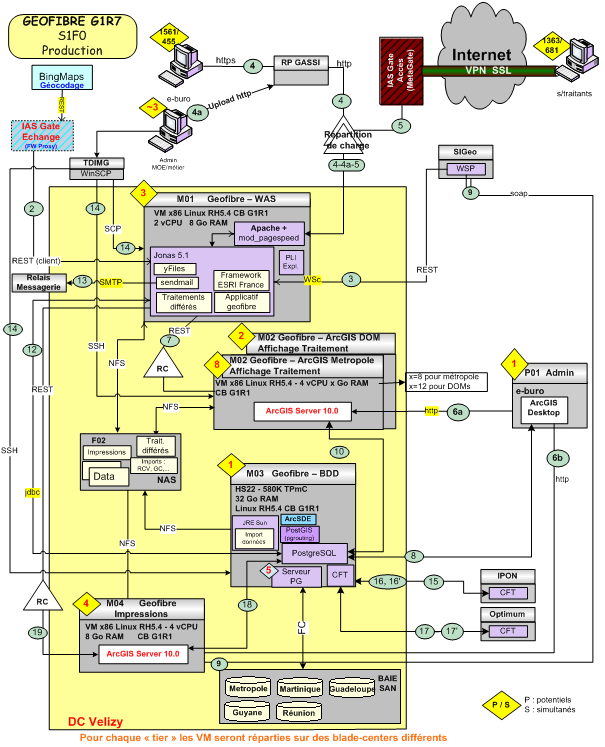
\includegraphics[width=16cm]{images/archtech.png}
  }
\end{figure}

\end{document}
